 %\documentclass[dvips]{beamer}
\documentclass{beamer}
\usepackage{amsmath,amssymb}
\usepackage{latexsym}
\usepackage{subfigure}
\usepackage{xspace}
\usepackage[colon]{natbib}

%\usetheme{Boadilla}
%\usepackage{natbib}
\usepackage{epstopdf}
\setbeamertemplate{footline}
\beamertemplatenavigationsymbolsempty
\usepackage{bm}
\AtBeginSection[]
{
 \begin{frame}
     \frametitle{Outline}
     \tableofcontents[currentsection]
 \end{frame}
}




%%%%%%%%%%%%%%%%%%%%%%%%%%%%%%%%%%%%%%%%%%%%%%%%%%%%%%%%%%%%%%%%%%


\newcommand{\Holder}{H\"older\xspace}
%\newcommand{\bm}{\mathbf}
\newcommand{\x}{x}
\renewcommand{\t}{\mathbf{t}}
\newcommand{\Zspace}{\mathcal{Z}}
\newcommand{\dataset}{\mathcal{D}}

\newcommand{\Bspace}{\mathcal{B}}
\newcommand{\f}{f}
\newcommand{\g}{g}
\newcommand{\h}{h}
\newcommand{\q}{q}
\newcommand{\I}{I}
\newcommand{\J}{J}
\newcommand{\entropy}{\mathcal{H}}
\newcommand{\jaak}{\lambda}
\newcommand{\trace}{\mathop{\textrm{tr}}}
\newcommand{\Trace}[1]{\mathop{\textrm{tr}}\left(#1\right)}

\newcommand{\diag}[1]{\mathop{\textrm{diag}}\left(#1\right)}
\newcommand{\D}{\mathcal{D}}

%\newcommand{\Z}{\mathcal{Z}}
\newcommand{\integral}{\mathcal{I}}
\newcommand{\tauspace}{\mathcal{T}}

\newcommand{\normdist}{\mathcal{N}}
\renewcommand{\r}{\Psi}
\newcommand{\s}{s}
\newcommand{\basem}{\nu}
\renewcommand{\L}{\Lambda}
\newcommand{\transp}{^{T}}

\newcommand{\red}[1]{{\color{red}#1}}

\newcommand{\LSE}[3]{\bar{\mathbb{E}}_{#1}^{#2}\left[#3\right]}
\newcommand{\unigint}[1]{{U}_{\left[#1\right]}}
%\newcommand{\Expectation}[2]{\mathbb{E}_{#1}\left[#2\right]}
\newcommand{\Expectation}[2]{\int{#2}d\nu(\Z)}
\newcommand{\Expectationsmall}[2]{\mathbb{E}_{#1}[#2]}
\newcommand{\Var}[2]{\textnormal{Var}_{#1}\left(#2\right)}
\newcommand{\Varsmall}[2]{\textnormal{Var}_{#1}(#2)}
\def\bin{\bar}
\def\idep{\perp\!\!\!\perp}
\def\Indic#1{\mathbb{I}_{\{#1\}}}
\def\w{\mathbf{w}}
\def\bx{\mathbf{x}}
\def\bz{\mathbf{z}}
%\def\Z{Z}
\def\u{\mathbf{u}}
\def\m{\mathbf{m}}
\def\s{\mathbf{s}}
\def\v{\mathbf{v}}
\def\T{T}
\def\A{A}
\def\bomega{\bm{\omega}}
\def\bbeta{{\bm{\beta}}}
\def\btau{{\bm{\tau}}}
\newcommand{\balpha}{{\bm{\alpha}}}

\def\X{X}
\def\Z{Z}
\def\z{z}
\def\p{p}

\def\bX{\bm{X}}
\def\y{\mathbf{y}}
%\def\dataset{\mathcal{D}}
\def\PG{\mathcal{PG}}

\def\eye{\mathbf{I}}
\def\bzeros{\mathbf{0}}

\def\proba{p}
%\def\m{\mathbf{m}}
%\def\v{\mathbf{v}}
%\def\a{\mathbf{a}}
%\def\b{\mathbf{b}}
\def\C{C}
\def\vect{\mathop{\textrm{vec}}}

\newcommand{\logit}{\mathsf{logit}}
\renewcommand{\Re}{\mathbb{R}}
\newcommand{\Rebar}{\bar\Re}

\newcommand{\vectorcat}[2]{\left(\begin{array}{c}#1\\#2\end{array}\right)}
\newcommand{\objective}{Z}
\newenvironment{prooflight}{\textsc{Proof (sketch)}\it}{$\Box$}
%\newenvironment{proof}{\textsc{proof.}\it}{\hfill{$\Box$}}

\newtheorem{proposition}{Proposition}

%%%%%%%%%%%%%%%%%%%%%%%%%%%%%%%%%%%%%%%%%%%%%%%%%%%%%%%%%%%%%%%%%%

\renewcommand{\emph}[1]{\textcolor{red}{\textbf{#1}}}
\title[Variational Holder Bound]{Approximate Inference with the \\ Variational \Holder Bound}
\author[Bouchard \& Lakshminarayanan]{Guillaume Bouchard \& Balaji Lakshminarayanan}
\date{\today}

\begin{document}
%\pgfdeclarelayer{background} \pgfsetlayers{background,main} 
\frame{\titlepage}

\section{Introduction}
%%%%%%%%%%%%%%%%%%%%%%%%%%%%%%%%%%%%%%%%%%%%%%%
\begin{frame}{Variational Inference}
	\begin{itemize}
	\item Many applications require computing large sums
		\begin{itemize}
		\item Decision under uncertainty
		\item Simulations
		\item Probabilistic Inference
		\end{itemize}
	\item Problem: most of the integrals are \emph{intractable}
	\item Goal: Find a \emph{tractable} approximation
	\end{itemize}
\end{frame}
%%%%%%%%%%%%%%%%%%%%%%%%%%%%%%%%%%%%%%%%%%%%%%%


%%%%%%%%%%%%%%%%%%%%%%%%%%%%%%%%%%%%%%%%%%%%%%%
\begin{frame}{Notations}
\begin{itemize}
	\item Unnormalized distribution: $\gamma(\Z) :=\gamma_1(\Z)\gamma_2(\Z)$.
	\item Partition function
	\begin{eqnarray}
	I^*:=\Expectation{}{\gamma_1(\Z)\gamma_2(\Z)}=\|\gamma_1\gamma_2\|_1
	\end{eqnarray}
	\item Normalized (target) distribution: $p^*(Z) := \frac{\gamma_1(\Z)\gamma_2(\Z)}{\|\gamma_1\gamma_2\|_1}$
\end{itemize}
\end{frame}
%%%%%%%%%%%%%%%%%%%%%%%%%%%%%%%%%%%%%%%%%%%%%%%


%%%%%%%%%%%%%%%%%%%%%%%%%%%%%%%%%%%%%%%%%%%%%%%
\begin{frame}{Lower Bound to $I^*$}
	\begin{eqnarray}
	\log I^*= \log \Expectation{}{\gamma_1(\Z)\gamma_2(\Z)}
	\\
	\ge \int \log\left\lbrace\gamma_1(\Z)\gamma_2(\Z)\right\rbrace d\nu(\Z)
	\end{eqnarray}
	By Jensen's inequality.
	
	This bound is not tight in general.
\end{frame}
%%%%%%%%%%%%%%%%%%%%%%%%%%%%%%%%%%%%%%%%%%%%%%%
%%%%%%%%%%%%%%%%%%%%%%%%%%%%%%%%%%%%%%%%%%%%%%%
\begin{frame}{Standard Variational Bayes}
	\begin{eqnarray}
	\log I^*= \log \int \frac{\gamma_1(\Z)\gamma_2(\Z)}{q(\Z)} d\q(\Z)
	\\
	\ge \int \log\left\lbrace \frac{\gamma_1(\Z)\gamma_2(\Z)}{q(\Z)} \right\rbrace d\q(\Z)
	\end{eqnarray}
	where $dq=\partial Q/\partial \nu$
	\begin{itemize}
		\item Bound \emph{maximized} w.~r.~t.~$\q$ (Variational inference)
		\item Tighter lower bound to the integral
		\item Not convex with respect to $Q$ in general
		\item Widely used
	\end{itemize}
	$\rightarrow$ We propose an alternative by \emph{minimizing} an upper bound
\end{frame}
%%%%%%%%%%%%%%%%%%%%%%%%%%%%%%%%%%%%%%%%%%%%%%%


\section{\Holder Variational Bayes}

%%%%%%%%%%%%%%%%%%%%%%%%%%%%%%%%%%%%%%%%%%%%%%%
\begin{frame}{Upper Bound to $I^*$}
	\begin{eqnarray}
	I^*= \Expectation{}{\gamma_1(\Z)\gamma_2(\Z)}
	\le 
	\sqrt{\int \gamma^2_1(\Z)d\nu(\Z)} 
	\sqrt{\int \gamma^2_2(\Z)d\nu(\Z)}
	\end{eqnarray}
	By \emph{Cauchy-Schwartz}'s inequality.
	
	This bound is not tight in general.
	
	\vspace{1cm}
	\textbf{Notation simplification}
	
	For short, we drop $\nu$ and $\Z$:
	\begin{eqnarray}
	I^*= \int \gamma_1\gamma_2
	\le 
	\sqrt{\int \gamma^2_1} 
	\sqrt{\int \gamma^2_2}
	\end{eqnarray}	
\end{frame}
%%%%%%%%%%%%%%%%%%%%%%%%%%%%%%%%%%%%%%%%%%%%%%%


%%%%%%%%%%%%%%%%%%%%%%%%%%%%%%%%%%%%%%%%%%%%%%%
\begin{frame}{Tighter Upper Bound to $I^*$}
	Cauchy-Schwartz's inequality is a special case of \emph{\Holder}'s inequality:
	
	\begin{eqnarray}
	I^*= \int \gamma_1\gamma_2
	\le 
	\left(\int \gamma^{\alpha_1}_1\right)^{\frac 1{\alpha_1}}
	\left(\int \gamma^{\alpha_2}_2\right)^{\frac 1{\alpha_2}}
	\end{eqnarray}
	For \Holder exponents $(\alpha_1,\alpha_2)$, i.e. $\frac 1{\alpha_1} + \frac 1{\alpha_2} = 1$
	
	This bound is better but not tight in general (unless $\gamma_1\equiv\gamma_2$).
	
	\vspace{1cm}
	$\rightarrow$ We use the variational tightening trick
\end{frame}
%%%%%%%%%%%%%%%%%%%%%%%%%%%%%%%%%%%%%%%%%%%%%%%



%%%%%%%%%%%%%%%%%%%%%%%%%%%%%%%%%%%%%%%%%%%%%%%
\begin{frame}{Variational \Holder  Bound}
	
	\begin{eqnarray}
	I^*&=& \int \gamma_1\gamma_2 = \int (\gamma_1\Psi) \frac{\gamma_2}{\Psi}
	\le \bar{I}_{\balpha}
	\\
	\bar{I}_{\balpha}(\Psi) &:=& \left(\int \gamma^{\alpha_1}_1 \Psi^{\alpha_1}\right)^{\frac 1{\alpha_1}}
	\left(\int \frac{\gamma^{\alpha_2}_2}{\Psi^{\alpha_2}}\right)^{\frac 1{\alpha_2}} \label{eq:vh}
	\end{eqnarray}
	For any $\Psi:\mathcal{Z}\mapsto\Re^+$ and any $\bm\alpha$ s.t. $\frac 1{\alpha_1} + \frac 1{\alpha_2} = 1$.
	
	Equality holds for $\Psi=\Psi^*\equiv\left(\frac{\gamma_2^{\alpha_2}}{\gamma_1^{\alpha_1}}\right)^{\frac{1}{\alpha_1+\alpha_2}} $.

	\begin{itemize}
		\item Bound \emph{minimized} w. r. t. $\Psi$ and $\balpha$ (Variational inference)
		\item Tighter upper bound to the integral
		\item log-\emph{convex} with respect to $\Psi$  %$\log\Psi$
		\item Generalization of previous use of \Holder's bound in binary graphical models~\citep{liu11d}
		\item Trade-off: Need to choose $\Psi$ such the bound is as tight as possible while still being able to optimize (\ref{eq:vh})  efficiently 
	\end{itemize}
	%$\rightarrow$ 
\end{frame}
%%%%%%%%%%%%%%%%%%%%%%%%%%%%%%%%%%%%%%%%%%%%%%%



%%%%%%%%%%%%%%%%%%%%%%%%%%%%%%%%%%%%%%%%%%%%%%%
\begin{frame}{Variational \Holder  Bayes}

	Parametric family of pivot functions: $\mathcal{F}=\{\Psi(.;\tau),\tau\in\tauspace\}$
	\begin{align}
	  (\hat\tau,\hat\alpha_1) \in \arg\min_{\tauspace\otimes\Re} \bar I_\balpha(\Psi(.,;\tau))
	\end{align}
	Resulting approximations of the posterior: 
	\begin{itemize}
	\item First tractable distribution:	
	\begin{eqnarray}
	\hat\proba_1(Z) := \frac{(\gamma_1(Z)\Psi(Z;\hat\btau))^{\alpha_1}}{\|\gamma_1\Psi(.;\hat\btau)\|^{\alpha_1}_{\alpha_1}}
	\end{eqnarray}
	\item Second tractable distribution:
	\begin{eqnarray}
	\hat\proba_2(Z) := \frac{(\gamma_2(Z)/\Psi(Z;\hat\btau))^{\alpha_2}}{\|\gamma_2/\Psi(.;\hat\btau)\|^{\alpha_2}_{\alpha_2}}
	\end{eqnarray}
	\item Mixture:
	\begin{eqnarray}
\hat\proba_{12}(Z) := \frac {1}{\alpha_1}\proba_1(Z) + \frac {1}{\alpha_2}\proba_2(Z)
\enspace
\end{eqnarray}	
	\end{itemize}
\end{frame}
%%%%%%%%%%%%%%%%%%%%%%%%%%%%%%%%%%%%%%%%%%%%%%%



\section{Application to Truncated Gaussian Integration}


%%%%%%%%%%%%%%%%%%%%%%%%%%%%%%%%%%%%%%%%%%%%%%%
\begin{frame}{Non-conjugate Gaussian Integration}

\begin{itemize}
	\item Quantity to compute:
		\begin{eqnarray} 
		I^*:=\int_{\Re^n}  \prod_{i=1}^n f_i(t_i)
		e^{-\frac 12 \t\transp \A \t + \bm b\transp \t} d\t
		\enspace.
		\label{univ-gaussian-integral} 
		\end{eqnarray}
	\item Common in machine learning~\citep{seeger2010gaussian}.
	\item Parts:
		\begin{enumerate}
		\item $\gamma_1(t)=\prod_{i=1}^n f_i(t_i)$ where  $f_i:\Re\mapsto \Re$ is univariate
		\item $\gamma_2(t)$ with $e^{-\frac 12 t\transp \A t + b\transp t}$, where $A\mathcal{S}_n^+$ and $\bm b\in\Re^n$.
		\end{enumerate}
	\item Pivot functions family $\{\Psi(\t;\btau) ,\btau\in\Re^{2n}\}$:
		\begin{eqnarray}
			\left\lbrace
				e^{-\frac 12 \t\transp\diag{\btau_1}\t +  \btau_2\transp\t},
				%\quad \btau = (\btau_1\transp,\btau_2\transp)\transp, 
				\quad \btau_1\in\Re^n,\btau_2 \in \Re^n 
			\right\rbrace
		.
		\label{Gaussian-pivot-functions}
		\end{eqnarray}
\end{itemize}
\end{frame}
%%%%%%%%%%%%%%%%%%%%%%%%%%%%%%%%%%%%%%%%%%%%%%%

%%%%%%%%%%%%%%%%%%%%%%%%%%%%%%%%%%%%%%%%%%%%%%%
\begin{frame}{Product of Univariate Functions}
	\begin{eqnarray} 
	\|\gamma_1\Psi(.,\btau)\|_{\alpha_1}^{\alpha_1}
	&=&
	%\int_{\Re^n} 
	%\prod_{i=1}^n f_i(t_i) 		e^{-\frac 12 \t\diag{\u_1} \t + \u_2\transp\t} d\t 
	%\nonumber\\
	%&=& 		
	\prod_{i=1}^n
	\int_\Re f_i^{\alpha_1}(t_i)
	e^{\alpha_1(-\frac{\tau_{1i} t_i^2}2 + \tau_{2i} t_i)}
	dt_i
	\nonumber\\
	&=&
	%= 
	\prod_{i=1}^n
	\unigint{f_i}\left(\tau_{1i},\tau_{2i},\alpha_1\right)
	\enspace,
	\label{ortho-univ}
	\end{eqnarray}
	Where the univariate integrals are:
	\begin{eqnarray}
	\unigint{h}(a,b,\alpha_1):=\int_\Re \left(h(t)e^{-\frac 12 a t^2 + b t}\right)^{\alpha_1} dt_i
	\enspace.
	\end{eqnarray} 
	Focus on truncated Gaussians: $f_i(x)=\Indic{x\ge 0}$ $\forall i\in\{1,\cdots,n\}$.
	
	$\rightarrow$ 	normal CDF function~$\Phi$:			
	\begin{eqnarray}
			\unigint{\Indic{\cdot\ge0}}(a,b,\alpha) 
			&		=		&
			\sqrt{\frac{2\pi}{\alpha a}} 
			  \Phi\left(b \sqrt{\frac{\alpha}{a}}\right)
	e^{\frac{\alpha b^2}{2 a}}
	\enspace.
\end{eqnarray}	

\end{frame}
%%%%%%%%%%%%%%%%%%%%%%%%%%%%%%%%%%%%%%%%%%%%%%%



%%%%%%%%%%%%%%%%%%%%%%%%%%%%%%%%%%%%%%%%%%%%%%%
\begin{frame}{Gaussian Integrals}
	\begin{flalign} 
	\|\gamma_2/\Psi(.,\btau)\|_{\alpha_2}^{\alpha_2}
	&=
	\int_{\Re^n} 
	e^{-\frac{\alpha_2}{2} \t\transp (\A - \diag{\btau_1}) \t + {\alpha_2}(\bm b - \btau_2)\transp \t} d\t
	\nonumber
	\\
	&= {(2\pi)^{\frac n2}}  e^{J\left(
			{\alpha_2}(A- \diag{\btau_1}),
			{\alpha_2}(\bm b - \btau_2)
		\right)},	
	\nonumber
	\end{flalign}
	where $J(M,v):=-\frac 12 \log |M| + \frac 12 v\transp M^{-1} v$.
\end{frame}
%%%%%%%%%%%%%%%%%%%%%%%%%%%%%%%%%%%%%%%%%%%%%%%


%%%%%%%%%%%%%%%%%%%%%%%%%%%%%%%%%%%%%%%%%%%%%%%
\begin{frame}{Experiments 2D Truncated Gaussians}
	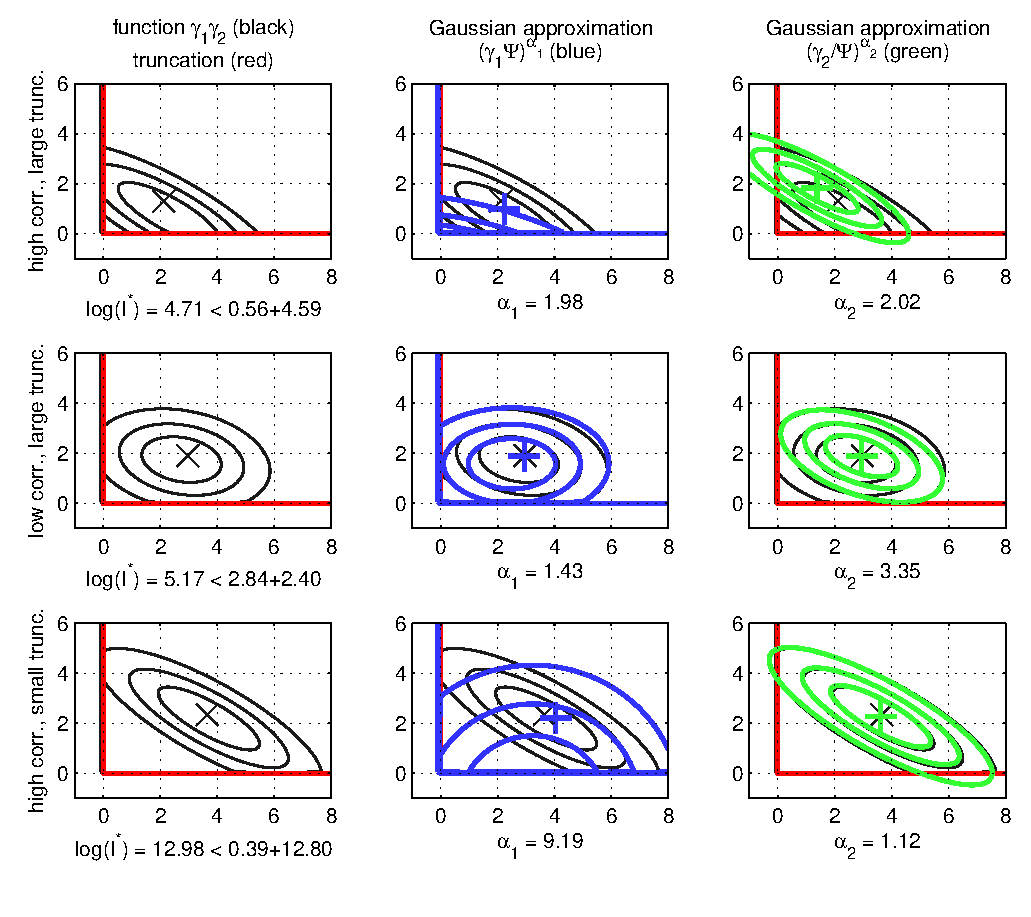
\includegraphics[width=.9\textwidth,, angle=0]{../pics/TruncGaussOrthant3_scissored.pdf}
%	\vspace{-1.2cm}
%	\small{2D Truncated Gaussian integration. Each row represents a different
%	correlation/truncation setting. From left to right, the columns show 
%	1) the
%	target function $\gamma_1\gamma_2$, 2) its first tractable approximation
%	$(\gamma_1\Psi)^{\alpha_1}$ (product of orthogonal univariate function) and 3)
%	its second tractable approximation $(\gamma_2/\Psi)^{\alpha_2}$ (correlated
%	Gaussian distribution). 
%	Symbols 'x' and '+' are the exact and approximate means, 
%	respectively.
%	}
\end{frame}
%%%%%%%%%%%%%%%%%%%%%%%%%%%%%%%%%%%%%%%%%%%%%%%


%%%%%%%%%%%%%%%%%%%%%%%%%%%%%%%%%%%%%%%%%%%%%%%
\begin{frame}{Experiments: Probit regression}
	\begin{itemize}
\item Generate $N=100$ data points as $x_m\sim \normdist(\rho y_m,1)$. % $w$ to $\normdist(0,1)$
\item The higher $\rho$, the more separable the two classes are	

\item Compare to Albert Chib auxiliary variable Gibbs sampler
\pause
\begin{table}[htdp]
\begin{center}
\resizebox{\columnwidth}{!}{
\begin{tabular}{|c|c|c|c|c|c|}
% $\dfrac{1}{\alpha_1}$
\hline
$\rho$ & $1/\alpha_1$ & $\bar\w_{1}$ & $\bar\w_{2}$ & $\bar\w_{12}$ (mix) & Gibbs $90\%$ CI \\
\hline
%0.1 & 0.875 & -0.575 & 0.82 & -0.4 & (0.7, 0.72)  \\
%0.25 &  0.868 & -1.89 & 1.23 & -1.48 &  (1.31, 1.35)  \\
0.5 & 0.869 & 2.03 & 2.54 & 2.09& (2.29, 2.43) \\
1 & 0.834 & 4.05 & 3.56 & 3.97 & (3.55, 3.59) \\
3 & 0.781 & 4.77 & 4.92  & 4.81& (4.8, 4.82) \\
10 & 0.769 & 4.93 & 5.1 & 4.97 & (5.04, 5.07) \\
\hline
\end{tabular}
}
\end{center}
%\caption{Results on one dimensional dataset.}% for varying $\rho$.}
\label{tab:toy1dall}
\end{table}%
\item Parameter estimates are slightly biased
\item As $\rho$ increases, the optimal value of $1/\alpha_1$ increases implying that the overall posterior is `more Gaussian'
	\end{itemize}
\end{frame}
%%%%%%%%%%%%%%%%%%%%%%%%%%%%%%%%%%%%%%%%%%%%%%%



\section{Theoretical Guarantees}

%%%%%%%%%%%%%%%%%%%%%%%%%%%%%%%%%%%%%%%%%%%%%%%
\begin{frame}{Approximation Guarantees}
\begin{proposition}  
\label{th:approx}
For any $\varepsilon>0$, the inequality $I^* > (1-\varepsilon) \bar I_\balpha(\Psi)$ implies that:
\begin{align}
\left\|
	\frac{(\gamma_1\Psi)^{\alpha_1}}{\|\gamma_1\Psi\|^{\alpha_1}_{\alpha_1}} 
	- 
	%\frac{\gamma_1\gamma_2}{\|\gamma_1\|_{\alpha_1}\|\gamma_2\|_{\alpha_2}} 	
	\proba^*
\right\|_2 < \sqrt{2\varepsilon} + \varepsilon
\quad &  \mathrm{if} \quad \alpha_1 \le 2, \mathrm{\ and}
\\
\left\|
	\frac{(\gamma_2/\Psi)^{\alpha_2}}{\|\gamma_2/\Psi\|^{\alpha_2}_{\alpha_2}} 
	- 
	%\frac{\gamma_1\gamma_2}{\|\gamma_1\|_{\alpha_1}\|\gamma_2\|_{\alpha_2}} 
	\proba^*
\right\|_2 < \sqrt{2\varepsilon} + \varepsilon
\quad  & \mathrm{if} \quad \alpha_1 \ge 2
\enspace.
\end{align}
\end{proposition} 

\end{frame}
%%%%%%%%%%%%%%%%%%%%%%%%%%%%%%%%%%%%%%%%%%%%%%%







\section{Conclusion and Future Work}
%%%%%%%%%%%%%%%%%%%%%%%%%%%%%%%%%%%%%%%%%%%%%%%
\begin{frame}{Conclusion}
	\begin{itemize}
	\item New variational inference scheme that involves convex optimization (global optima, easy to assess convergence)
	\item Approximation guarantees (unknown for Jensen-VB)
	\item Applied to truncated Gaussian integration $\rightarrow$ Probit regression.
	\item Generalization of Tree-Reweighted (TRW) bound 
		\item Disclaimer: Upper bound is not good for multi-modal posterior (e.g. clustering)
	\end{itemize}
\end{frame}
%%%%%%%%%%%%%%%%%%%%%%%%%%%%%%%%%%%%%%%%%%%%%%%

%%%%%%%%%%%%%%%%%%%%%%%%%%%%%%%%%%%%%%%%%%%%%%%
\begin{frame}{Future work}
	\begin{itemize}
	\item Large scale experimental validation with comparison to VB, EP and sampling
	\item Apply VH to Polya-Gamma Bayesian logistic regression
	\item Apply VH for convex Bayesian matrix factorization		
	\item Apply VH for high-order potentials, such as PCFG $\times$ Markov models			
	\item Show that VH is a Generalization of Tree-Reweighted (TRW) bound when there is one spanning tree per factor
	\end{itemize}
\end{frame}
%%%%%%%%%%%%%%%%%%%%%%%%%%%%%%%%%%%%%%%%%%%%%%%


%%%%%%%%%%%%%%%%%%%%%%%%%%%%%%%%%%%%%%%%%%%%%%%
%\bibliographystyle{plainnat}
\begin{frame}{References}
\bibliographystyle{apalike}
\bibliography{vh_bib}
\end{frame}
\end{document}


%%%%%%%%%%%%%%%%%%%%%%%%%%%%%%%%%%%%%%%%%%%%%%%
%\begin{frame}{title}
%	\begin{itemize}
%	\item a
%	\item b
%	\end{itemize}
%\end{frame}
%%%%%%%%%%%%%%%%%%%%%%%%%%%%%%%%%%%%%%%%%%%%%%%

